\documentclass[1p]{elsarticle_modified}
%\bibliographystyle{elsarticle-num}

%\usepackage[colorlinks]{hyperref}
%\usepackage{abbrmath_seonhwa} %\Abb, \Ascr, \Acal ,\Abf, \Afrak
\usepackage{amsfonts}
\usepackage{amssymb}
\usepackage{amsmath}
\usepackage{amsthm}
\usepackage{scalefnt}
\usepackage{amsbsy}
\usepackage{kotex}
\usepackage{caption}
\usepackage{subfig}
\usepackage{color}
\usepackage{graphicx}
\usepackage{xcolor} %% white, black, red, green, blue, cyan, magenta, yellow
\usepackage{float}
\usepackage{setspace}
\usepackage{hyperref}

\usepackage{tikz}
\usetikzlibrary{arrows}

\usepackage{multirow}
\usepackage{array} % fixed length table
\usepackage{hhline}

%%%%%%%%%%%%%%%%%%%%%
\makeatletter
\renewcommand*\env@matrix[1][\arraystretch]{%
	\edef\arraystretch{#1}%
	\hskip -\arraycolsep
	\let\@ifnextchar\new@ifnextchar
	\array{*\c@MaxMatrixCols c}}
\makeatother %https://tex.stackexchange.com/questions/14071/how-can-i-increase-the-line-spacing-in-a-matrix
%%%%%%%%%%%%%%%

\usepackage[normalem]{ulem}

\newcommand{\msout}[1]{\ifmmode\text{\sout{\ensuremath{#1}}}\else\sout{#1}\fi}
%SOURCE: \msout is \stkout macro in https://tex.stackexchange.com/questions/20609/strikeout-in-math-mode

\newcommand{\cancel}[1]{
	\ifmmode
	{\color{red}\msout{#1}}
	\else
	{\color{red}\sout{#1}}
	\fi
}

\newcommand{\add}[1]{
	{\color{blue}\uwave{#1}}
}

\newcommand{\replace}[2]{
	\ifmmode
	{\color{red}\msout{#1}}{\color{blue}\uwave{#2}}
	\else
	{\color{red}\sout{#1}}{\color{blue}\uwave{#2}}
	\fi
}

\newcommand{\Sol}{\mathcal{S}} %segment
\newcommand{\D}{D} %diagram
\newcommand{\A}{\mathcal{A}} %arc


%%%%%%%%%%%%%%%%%%%%%%%%%%%%%5 test

\def\sl{\operatorname{\textup{SL}}(2,\Cbb)}
\def\psl{\operatorname{\textup{PSL}}(2,\Cbb)}
\def\quan{\mkern 1mu \triangleright \mkern 1mu}

\theoremstyle{definition}
\newtheorem{thm}{Theorem}[section]
\newtheorem{prop}[thm]{Proposition}
\newtheorem{lem}[thm]{Lemma}
\newtheorem{ques}[thm]{Question}
\newtheorem{cor}[thm]{Corollary}
\newtheorem{defn}[thm]{Definition}
\newtheorem{exam}[thm]{Example}
\newtheorem{rmk}[thm]{Remark}
\newtheorem{alg}[thm]{Algorithm}

\newcommand{\I}{\sqrt{-1}}
\begin{document}

%\begin{frontmatter}
%
%\title{Boundary parabolic representations of knots up to 8 crossings}
%
%%% Group authors per affiliation:
%\author{Yunhi Cho} 
%\address{Department of Mathematics, University of Seoul, Seoul, Korea}
%\ead{yhcho@uos.ac.kr}
%
%
%\author{Seonhwa Kim} %\fnref{s_kim}}
%\address{Center for Geometry and Physics, Institute for Basic Science, Pohang, 37673, Korea}
%\ead{ryeona17@ibs.re.kr}
%
%\author{Hyuk Kim}
%\address{Department of Mathematical Sciences, Seoul National University, Seoul 08826, Korea}
%\ead{hyukkim@snu.ac.kr}
%
%\author{Seokbeom Yoon}
%\address{Department of Mathematical Sciences, Seoul National University, Seoul, 08826,  Korea}
%\ead{sbyoon15@snu.ac.kr}
%
%\begin{abstract}
%We find all boundary parabolic representation of knots up to 8 crossings.
%
%\end{abstract}
%\begin{keyword}
%    \MSC[2010] 57M25 
%\end{keyword}
%
%\end{frontmatter}

%\linenumbers
%\tableofcontents
%
\newcommand\colored[1]{\textcolor{white}{\rule[-0.35ex]{0.8em}{1.4ex}}\kern-0.8em\color{red} #1}%
%\newcommand\colored[1]{\textcolor{white}{ #1}\kern-2.17ex	\textcolor{white}{ #1}\kern-1.81ex	\textcolor{white}{ #1}\kern-2.15ex\color{red}#1	}

{\Large $\underline{12n_{0382}~(K12n_{0382})}$}

\setlength{\tabcolsep}{10pt}
\renewcommand{\arraystretch}{1.6}
\vspace{1cm}\begin{tabular}{m{100pt}>{\centering\arraybackslash}m{274pt}}
\multirow{5}{120pt}{
	\centering
	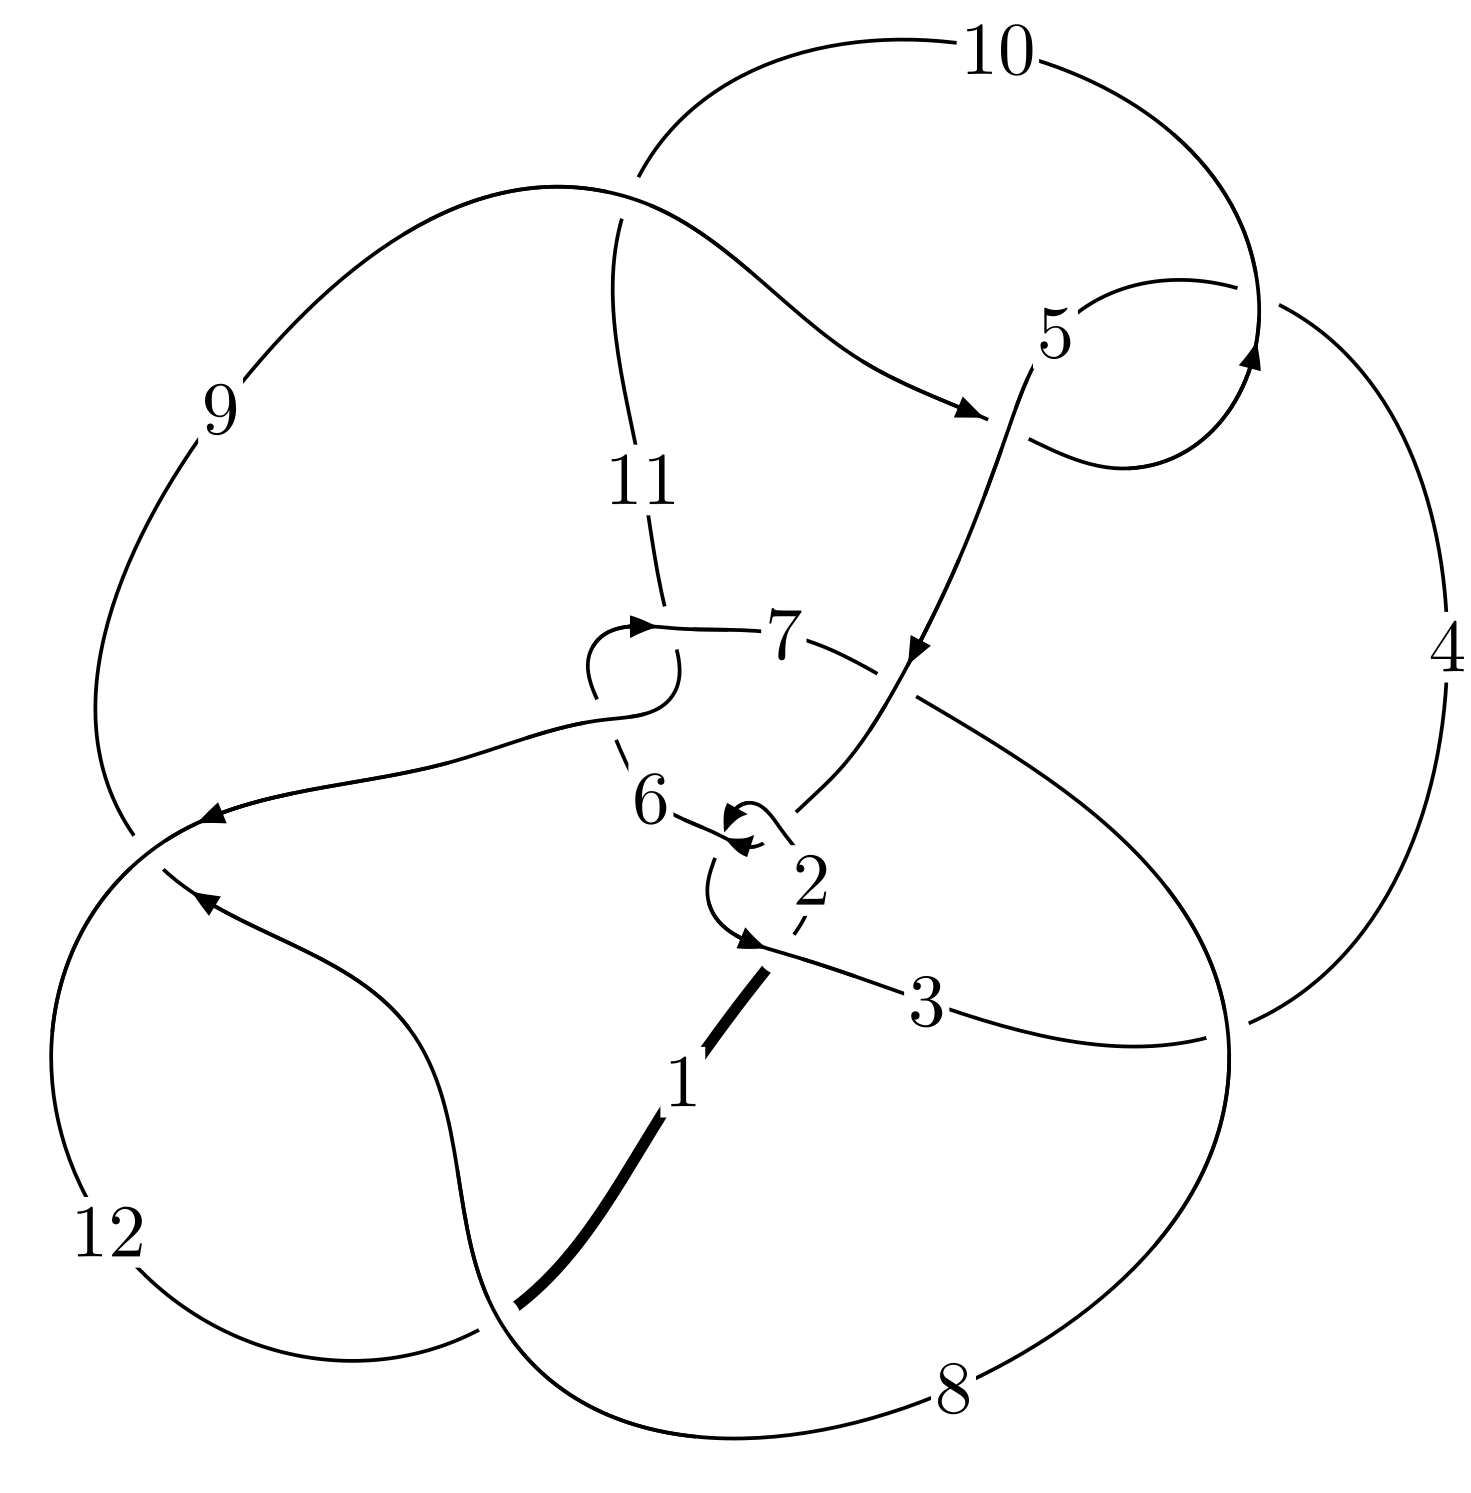
\includegraphics[width=112pt]{../../../GIT/diagram.site/Diagrams/png/2471_12n_0382.png}\\
\ \ \ A knot diagram\footnotemark}&
\allowdisplaybreaks
\textbf{Linearized knot diagam} \\
\cline{2-2}
 &
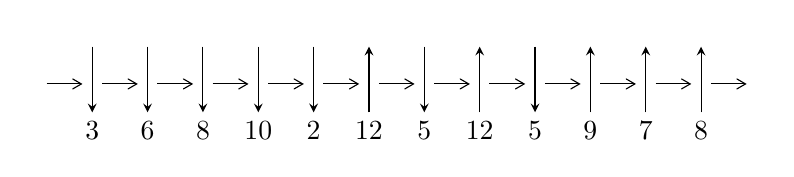
\begin{tikzpicture}[x=20pt, y=17pt]
	% nodes
	\node (C0) at (0, 0) {};
	\node (C1) at (1, 0) {};
	\node (C1U) at (1, +1) {};
	\node (C1D) at (1, -1) {3};

	\node (C2) at (2, 0) {};
	\node (C2U) at (2, +1) {};
	\node (C2D) at (2, -1) {6};

	\node (C3) at (3, 0) {};
	\node (C3U) at (3, +1) {};
	\node (C3D) at (3, -1) {8};

	\node (C4) at (4, 0) {};
	\node (C4U) at (4, +1) {};
	\node (C4D) at (4, -1) {10};

	\node (C5) at (5, 0) {};
	\node (C5U) at (5, +1) {};
	\node (C5D) at (5, -1) {2};

	\node (C6) at (6, 0) {};
	\node (C6U) at (6, +1) {};
	\node (C6D) at (6, -1) {12};

	\node (C7) at (7, 0) {};
	\node (C7U) at (7, +1) {};
	\node (C7D) at (7, -1) {5};

	\node (C8) at (8, 0) {};
	\node (C8U) at (8, +1) {};
	\node (C8D) at (8, -1) {12};

	\node (C9) at (9, 0) {};
	\node (C9U) at (9, +1) {};
	\node (C9D) at (9, -1) {5};

	\node (C10) at (10, 0) {};
	\node (C10U) at (10, +1) {};
	\node (C10D) at (10, -1) {9};

	\node (C11) at (11, 0) {};
	\node (C11U) at (11, +1) {};
	\node (C11D) at (11, -1) {7};

	\node (C12) at (12, 0) {};
	\node (C12U) at (12, +1) {};
	\node (C12D) at (12, -1) {8};
	\node (C13) at (13, 0) {};

	% arrows
	\draw[->,>={angle 60}]
	(C0) edge (C1) (C1) edge (C2) (C2) edge (C3) (C3) edge (C4) (C4) edge (C5) (C5) edge (C6) (C6) edge (C7) (C7) edge (C8) (C8) edge (C9) (C9) edge (C10) (C10) edge (C11) (C11) edge (C12) (C12) edge (C13) ;	\draw[->,>=stealth]
	(C1U) edge (C1D) (C2U) edge (C2D) (C3U) edge (C3D) (C4U) edge (C4D) (C5U) edge (C5D) (C6D) edge (C6U) (C7U) edge (C7D) (C8D) edge (C8U) (C9U) edge (C9D) (C10D) edge (C10U) (C11D) edge (C11U) (C12D) edge (C12U) ;
	\end{tikzpicture} \\
\hhline{~~} \\& 
\textbf{Solving Sequence} \\ \cline{2-2} 
 &
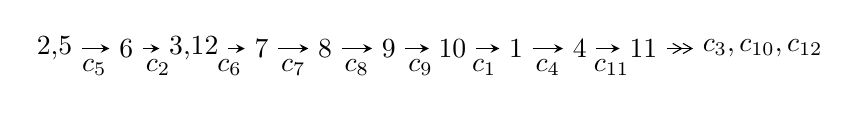
\begin{tikzpicture}[x=23pt, y=7pt]
	% node
	\node (A0) at (-1/8, 0) {2,5};
	\node (A1) at (1, 0) {6};
	\node (A2) at (33/16, 0) {3,12};
	\node (A3) at (25/8, 0) {7};
	\node (A4) at (33/8, 0) {8};
	\node (A5) at (41/8, 0) {9};
	\node (A6) at (49/8, 0) {10};
	\node (A7) at (57/8, 0) {1};
	\node (A8) at (65/8, 0) {4};
	\node (A9) at (73/8, 0) {11};
	\node (C1) at (1/2, -1) {$c_{5}$};
	\node (C2) at (3/2, -1) {$c_{2}$};
	\node (C3) at (21/8, -1) {$c_{6}$};
	\node (C4) at (29/8, -1) {$c_{7}$};
	\node (C5) at (37/8, -1) {$c_{8}$};
	\node (C6) at (45/8, -1) {$c_{9}$};
	\node (C7) at (53/8, -1) {$c_{1}$};
	\node (C8) at (61/8, -1) {$c_{4}$};
	\node (C9) at (69/8, -1) {$c_{11}$};
	\node (A10) at (11, 0) {$c_{3},c_{10},c_{12}$};

	% edge
	\draw[->,>=stealth]	
	(A0) edge (A1) (A1) edge (A2) (A2) edge (A3) (A3) edge (A4) (A4) edge (A5) (A5) edge (A6) (A6) edge (A7) (A7) edge (A8) (A8) edge (A9) ;
	\draw[->>,>={angle 60}]	
	(A9) edge (A10);
\end{tikzpicture} \\ 

\end{tabular} \\

\footnotetext{
The image of knot diagram is generated by the software ``\textbf{Draw programme}" developed by Andrew Bartholomew(\url{http://www.layer8.co.uk/maths/draw/index.htm\#Running-draw}), where we modified some parts for our purpose(\url{https://github.com/CATsTAILs/LinksPainter}).
}\phantom \\ \newline 
\centering \textbf{Ideals for irreducible components\footnotemark of $X_{\text{par}}$} 
 
\begin{align*}
I^u_{1}&=\langle 
-579753405694973 u^{23}-472990592837092 u^{22}+\cdots+1971269389223473 b+4407120302352329,\\
\phantom{I^u_{1}}&\phantom{= \langle  }2.83690\times10^{15} u^{23}+6.39000\times10^{15} u^{22}+\cdots+2.16840\times10^{16} a-5.46780\times10^{16},\;u^{24}+2 u^{23}+\cdots-7 u-11\rangle \\
I^u_{2}&=\langle 
- u^{14}+u^{13}+3 u^{12}-4 u^{11}-6 u^{10}+9 u^9+7 u^8-13 u^7-6 u^6+12 u^5+2 u^4-7 u^3+b+u,\\
\phantom{I^u_{2}}&\phantom{= \langle  }-2 u^{14}+u^{13}+5 u^{12}-4 u^{11}-10 u^{10}+8 u^9+10 u^8-10 u^7-8 u^6+7 u^5-2 u^3+u^2+a- u,\\
\phantom{I^u_{2}}&\phantom{= \langle  }u^{15}- u^{14}-3 u^{13}+4 u^{12}+6 u^{11}-9 u^{10}-7 u^9+13 u^8+6 u^7-13 u^6-2 u^5+8 u^4-3 u^2+1\rangle \\
\\
\end{align*}
\raggedright * 2 irreducible components of $\dim_{\mathbb{C}}=0$, with total 39 representations.\\
\footnotetext{All coefficients of polynomials are rational numbers. But the coefficients are sometimes approximated in decimal forms when there is not enough margin.}
\newpage
\renewcommand{\arraystretch}{1}
\centering \section*{I. $I^u_{1}= \langle -5.80\times10^{14} u^{23}-4.73\times10^{14} u^{22}+\cdots+1.97\times10^{15} b+4.41\times10^{15},\;2.84\times10^{15} u^{23}+6.39\times10^{15} u^{22}+\cdots+2.17\times10^{16} a-5.47\times10^{16},\;u^{24}+2 u^{23}+\cdots-7 u-11 \rangle$}
\flushleft \textbf{(i) Arc colorings}\\
\begin{tabular}{m{7pt} m{180pt} m{7pt} m{180pt} }
\flushright $a_{2}=$&$\begin{pmatrix}0\\u\end{pmatrix}$ \\
\flushright $a_{5}=$&$\begin{pmatrix}1\\0\end{pmatrix}$ \\
\flushright $a_{6}=$&$\begin{pmatrix}1\\u^2\end{pmatrix}$ \\
\flushright $a_{3}=$&$\begin{pmatrix}- u\\- u^3+u\end{pmatrix}$ \\
\flushright $a_{12}=$&$\begin{pmatrix}-0.130829 u^{23}-0.294688 u^{22}+\cdots-1.59763 u+2.52159\\0.294102 u^{23}+0.239942 u^{22}+\cdots+0.00494916 u-2.23568\end{pmatrix}$ \\
\flushright $a_{7}=$&$\begin{pmatrix}-0.534965 u^{23}-0.416078 u^{22}+\cdots-0.624684 u+5.43098\\-0.310244 u^{23}-0.272323 u^{22}+\cdots-0.324549 u+2.64692\end{pmatrix}$ \\
\flushright $a_{8}=$&$\begin{pmatrix}-0.224721 u^{23}-0.143755 u^{22}+\cdots-0.300135 u+2.78406\\-0.310244 u^{23}-0.272323 u^{22}+\cdots-0.324549 u+2.64692\end{pmatrix}$ \\
\flushright $a_{9}=$&$\begin{pmatrix}0.201549 u^{23}+0.249559 u^{22}+\cdots-0.113316 u-1.36979\\-0.111431 u^{23}-0.128131 u^{22}+\cdots-0.277454 u+1.05051\end{pmatrix}$ \\
\flushright $a_{10}=$&$\begin{pmatrix}0.312979 u^{23}+0.377690 u^{22}+\cdots+0.164138 u-2.42030\\-0.111431 u^{23}-0.128131 u^{22}+\cdots-0.277454 u+1.05051\end{pmatrix}$ \\
\flushright $a_{1}=$&$\begin{pmatrix}u^3\\u^5- u^3+u\end{pmatrix}$ \\
\flushright $a_{4}=$&$\begin{pmatrix}0.0617504 u^{23}-0.0392309 u^{22}+\cdots-2.06682 u+0.542106\\0.194220 u^{23}+0.176940 u^{22}+\cdots+0.957672 u-1.78638\end{pmatrix}$ \\
\flushright $a_{11}=$&$\begin{pmatrix}-0.0302642 u^{23}+0.0123334 u^{22}+\cdots+0.976733 u-1.03269\\0.119247 u^{23}+0.191200 u^{22}+\cdots+0.994406 u-1.82283\end{pmatrix}$\\&\end{tabular}
\flushleft \textbf{(ii) Obstruction class $= -1$}\\~\\
\flushleft \textbf{(iii) Cusp Shapes $= \frac{2580377549362014}{1971269389223473} u^{23}+\frac{3507150554528052}{1971269389223473} u^{22}+\cdots+\frac{45898132692487883}{1971269389223473} u-\frac{44289338047701926}{1971269389223473}$}\\~\\
\newpage\renewcommand{\arraystretch}{1}
\flushleft \textbf{(iv) u-Polynomials at the component}\newline \\
\begin{tabular}{m{50pt}|m{274pt}}
Crossings & \hspace{64pt}u-Polynomials at each crossing \\
\hline $$\begin{aligned}c_{1}\end{aligned}$$&$\begin{aligned}
&u^{24}+16 u^{23}+\cdots+819 u+121
\end{aligned}$\\
\hline $$\begin{aligned}c_{2},c_{5}\end{aligned}$$&$\begin{aligned}
&u^{24}+2 u^{23}+\cdots-7 u-11
\end{aligned}$\\
\hline $$\begin{aligned}c_{3}\end{aligned}$$&$\begin{aligned}
&u^{24}+26 u^{22}+\cdots+39 u-11
\end{aligned}$\\
\hline $$\begin{aligned}c_{4},c_{9}\end{aligned}$$&$\begin{aligned}
&u^{24}+u^{23}+\cdots+51 u+43
\end{aligned}$\\
\hline $$\begin{aligned}c_{6},c_{11}\end{aligned}$$&$\begin{aligned}
&u^{24}-2 u^{23}+\cdots-472 u-163
\end{aligned}$\\
\hline $$\begin{aligned}c_{7}\end{aligned}$$&$\begin{aligned}
&u^{24}-3 u^{23}+\cdots+9 u+1
\end{aligned}$\\
\hline $$\begin{aligned}c_{8},c_{12}\end{aligned}$$&$\begin{aligned}
&u^{24}+4 u^{23}+\cdots-138 u-23
\end{aligned}$\\
\hline $$\begin{aligned}c_{10}\end{aligned}$$&$\begin{aligned}
&u^{24}-7 u^{23}+\cdots-667 u+1849
\end{aligned}$\\
\hline
\end{tabular}\\~\\
\newpage\renewcommand{\arraystretch}{1}
\flushleft \textbf{(v) Riley Polynomials at the component}\newline \\
\begin{tabular}{m{50pt}|m{274pt}}
Crossings & \hspace{64pt}Riley Polynomials at each crossing \\
\hline $$\begin{aligned}c_{1}\end{aligned}$$&$\begin{aligned}
&y^{24}-8 y^{23}+\cdots+75809 y+14641
\end{aligned}$\\
\hline $$\begin{aligned}c_{2},c_{5}\end{aligned}$$&$\begin{aligned}
&y^{24}-16 y^{23}+\cdots-819 y+121
\end{aligned}$\\
\hline $$\begin{aligned}c_{3}\end{aligned}$$&$\begin{aligned}
&y^{24}+52 y^{23}+\cdots-1015 y+121
\end{aligned}$\\
\hline $$\begin{aligned}c_{4},c_{9}\end{aligned}$$&$\begin{aligned}
&y^{24}+7 y^{23}+\cdots+667 y+1849
\end{aligned}$\\
\hline $$\begin{aligned}c_{6},c_{11}\end{aligned}$$&$\begin{aligned}
&y^{24}+36 y^{23}+\cdots-234846 y+26569
\end{aligned}$\\
\hline $$\begin{aligned}c_{7}\end{aligned}$$&$\begin{aligned}
&y^{24}-47 y^{23}+\cdots+113 y+1
\end{aligned}$\\
\hline $$\begin{aligned}c_{8},c_{12}\end{aligned}$$&$\begin{aligned}
&y^{24}+34 y^{23}+\cdots-65412 y+529
\end{aligned}$\\
\hline $$\begin{aligned}c_{10}\end{aligned}$$&$\begin{aligned}
&y^{24}+35 y^{23}+\cdots-209766481 y+3418801
\end{aligned}$\\
\hline
\end{tabular}\\~\\
\newpage\flushleft \textbf{(vi) Complex Volumes and Cusp Shapes}
$$\begin{array}{c|c|c}  
\text{Solutions to }I^u_{1}& \I (\text{vol} + \sqrt{-1}CS) & \text{Cusp shape}\\
 \hline 
\begin{aligned}
u &= -0.840681 + 0.490024 I \\
a &= -0.724162 + 0.569771 I \\
b &= -0.34121 + 1.49688 I\end{aligned}
 & -2.96579 + 0.05300 I & -5.61914 - 0.01464 I \\ \hline\begin{aligned}
u &= -0.840681 - 0.490024 I \\
a &= -0.724162 - 0.569771 I \\
b &= -0.34121 - 1.49688 I\end{aligned}
 & -2.96579 - 0.05300 I & -5.61914 + 0.01464 I \\ \hline\begin{aligned}
u &= -1.022560 + 0.295401 I \\
a &= -1.05742 + 2.52587 I \\
b &= \phantom{-}0.33303 + 1.71764 I\end{aligned}
 & -3.54040 + 2.95826 I & -5.57765 - 4.27465 I \\ \hline\begin{aligned}
u &= -1.022560 - 0.295401 I \\
a &= -1.05742 - 2.52587 I \\
b &= \phantom{-}0.33303 - 1.71764 I\end{aligned}
 & -3.54040 - 2.95826 I & -5.57765 + 4.27465 I \\ \hline\begin{aligned}
u &= \phantom{-}0.962010 + 0.650431 I \\
a &= -0.070965 - 1.233660 I \\
b &= -0.070549 - 0.869894 I\end{aligned}
 & \phantom{-}7.79911 - 2.52001 I & -0.51262 + 2.53374 I \\ \hline\begin{aligned}
u &= \phantom{-}0.962010 - 0.650431 I \\
a &= -0.070965 + 1.233660 I \\
b &= -0.070549 + 0.869894 I\end{aligned}
 & \phantom{-}7.79911 + 2.52001 I & -0.51262 - 2.53374 I \\ \hline\begin{aligned}
u &= -0.927407 + 0.744557 I \\
a &= \phantom{-}0.713189 + 0.275798 I \\
b &= -0.014139 - 0.602418 I\end{aligned}
 & \phantom{-}8.76252 + 2.82949 I & -3.38778 - 2.96422 I \\ \hline\begin{aligned}
u &= -0.927407 - 0.744557 I \\
a &= \phantom{-}0.713189 - 0.275798 I \\
b &= -0.014139 + 0.602418 I\end{aligned}
 & \phantom{-}8.76252 - 2.82949 I & -3.38778 + 2.96422 I \\ \hline\begin{aligned}
u &= \phantom{-}1.133700 + 0.502318 I \\
a &= \phantom{-}0.53485 + 1.45879 I \\
b &= -1.02104 + 1.23446 I\end{aligned}
 & -2.58040 - 6.55097 I & -3.00232 + 8.95233 I \\ \hline\begin{aligned}
u &= \phantom{-}1.133700 - 0.502318 I \\
a &= \phantom{-}0.53485 - 1.45879 I \\
b &= -1.02104 - 1.23446 I\end{aligned}
 & -2.58040 + 6.55097 I & -3.00232 - 8.95233 I\\
 \hline 
 \end{array}$$\newpage$$\begin{array}{c|c|c}  
\text{Solutions to }I^u_{1}& \I (\text{vol} + \sqrt{-1}CS) & \text{Cusp shape}\\
 \hline 
\begin{aligned}
u &= -0.759420\phantom{ +0.000000I} \\
a &= -0.396801\phantom{ +0.000000I} \\
b &= -0.537831\phantom{ +0.000000I}\end{aligned}
 & -1.01372\phantom{ +0.000000I} & -11.2860\phantom{ +0.000000I} \\ \hline\begin{aligned}
u &= -0.238482 + 1.223910 I \\
a &= \phantom{-}0.037299 - 0.531429 I \\
b &= \phantom{-}0.12489 - 1.74552 I\end{aligned}
 & -9.56824 - 4.63986 I & -2.53665 + 1.77990 I \\ \hline\begin{aligned}
u &= -0.238482 - 1.223910 I \\
a &= \phantom{-}0.037299 + 0.531429 I \\
b &= \phantom{-}0.12489 + 1.74552 I\end{aligned}
 & -9.56824 + 4.63986 I & -2.53665 - 1.77990 I \\ \hline\begin{aligned}
u &= \phantom{-}1.25828\phantom{ +0.000000I} \\
a &= -1.11711\phantom{ +0.000000I} \\
b &= \phantom{-}0.135805\phantom{ +0.000000I}\end{aligned}
 & -0.844274\phantom{ +0.000000I} & -6.82360\phantom{ +0.000000I} \\ \hline\begin{aligned}
u &= \phantom{-}0.264664 + 0.670266 I \\
a &= -0.018243 - 0.736439 I \\
b &= \phantom{-}0.587531 + 0.857775 I\end{aligned}
 & -0.06550 + 2.02589 I & \phantom{-}0.03613 - 4.27604 I \\ \hline\begin{aligned}
u &= \phantom{-}0.264664 - 0.670266 I \\
a &= -0.018243 + 0.736439 I \\
b &= \phantom{-}0.587531 - 0.857775 I\end{aligned}
 & -0.06550 - 2.02589 I & \phantom{-}0.03613 + 4.27604 I \\ \hline\begin{aligned}
u &= -1.330090 + 0.222342 I \\
a &= -0.92490 + 1.09593 I \\
b &= \phantom{-}0.094519 + 1.136320 I\end{aligned}
 & -4.70867 + 0.81596 I & -5.59655 - 0.54882 I \\ \hline\begin{aligned}
u &= -1.330090 - 0.222342 I \\
a &= -0.92490 - 1.09593 I \\
b &= \phantom{-}0.094519 - 1.136320 I\end{aligned}
 & -4.70867 - 0.81596 I & -5.59655 + 0.54882 I \\ \hline\begin{aligned}
u &= \phantom{-}0.538622 + 0.352121 I \\
a &= \phantom{-}0.147046 + 1.001000 I \\
b &= \phantom{-}0.216583 - 0.106477 I\end{aligned}
 & \phantom{-}0.98010 - 1.26540 I & \phantom{-}3.01329 + 5.29615 I \\ \hline\begin{aligned}
u &= \phantom{-}0.538622 - 0.352121 I \\
a &= \phantom{-}0.147046 - 1.001000 I \\
b &= \phantom{-}0.216583 + 0.106477 I\end{aligned}
 & \phantom{-}0.98010 + 1.26540 I & \phantom{-}3.01329 - 5.29615 I\\
 \hline 
 \end{array}$$\newpage$$\begin{array}{c|c|c}  
\text{Solutions to }I^u_{1}& \I (\text{vol} + \sqrt{-1}CS) & \text{Cusp shape}\\
 \hline 
\begin{aligned}
u &= -1.34887 + 0.69749 I \\
a &= \phantom{-}1.08996 - 1.58558 I \\
b &= -0.23003 - 1.81299 I\end{aligned}
 & -13.0253 + 11.4321 I & -3.86498 - 4.79478 I \\ \hline\begin{aligned}
u &= -1.34887 - 0.69749 I \\
a &= \phantom{-}1.08996 + 1.58558 I \\
b &= -0.23003 + 1.81299 I\end{aligned}
 & -13.0253 - 11.4321 I & -3.86498 + 4.79478 I \\ \hline\begin{aligned}
u &= \phantom{-}1.55966 + 0.42079 I \\
a &= -0.69697 - 1.79236 I \\
b &= \phantom{-}0.02142 - 1.78671 I\end{aligned}
 & -15.5246 - 1.3214 I & -5.39704 + 0.62510 I \\ \hline\begin{aligned}
u &= \phantom{-}1.55966 - 0.42079 I \\
a &= -0.69697 + 1.79236 I \\
b &= \phantom{-}0.02142 + 1.78671 I\end{aligned}
 & -15.5246 + 1.3214 I & -5.39704 - 0.62510 I\\
 \hline 
 \end{array}$$\newpage\newpage\renewcommand{\arraystretch}{1}
\centering \section*{II. $I^u_{2}= \langle - u^{14}+u^{13}+\cdots+b+u,\;-2 u^{14}+u^{13}+\cdots+a- u,\;u^{15}- u^{14}+\cdots-3 u^2+1 \rangle$}
\flushleft \textbf{(i) Arc colorings}\\
\begin{tabular}{m{7pt} m{180pt} m{7pt} m{180pt} }
\flushright $a_{2}=$&$\begin{pmatrix}0\\u\end{pmatrix}$ \\
\flushright $a_{5}=$&$\begin{pmatrix}1\\0\end{pmatrix}$ \\
\flushright $a_{6}=$&$\begin{pmatrix}1\\u^2\end{pmatrix}$ \\
\flushright $a_{3}=$&$\begin{pmatrix}- u\\- u^3+u\end{pmatrix}$ \\
\flushright $a_{12}=$&$\begin{pmatrix}2 u^{14}- u^{13}+\cdots- u^2+u\\u^{14}- u^{13}+\cdots+7 u^3- u\end{pmatrix}$ \\
\flushright $a_{7}=$&$\begin{pmatrix}- u^{14}- u^{13}+\cdots- u+3\\- u^{12}+3 u^{10}- u^9-6 u^8+2 u^7+7 u^6-3 u^5-6 u^4+2 u^3+2 u^2- u\end{pmatrix}$ \\
\flushright $a_{8}=$&$\begin{pmatrix}- u^{14}- u^{13}+\cdots-9 u^2+3\\- u^{12}+3 u^{10}- u^9-6 u^8+2 u^7+7 u^6-3 u^5-6 u^4+2 u^3+2 u^2- u\end{pmatrix}$ \\
\flushright $a_{9}=$&$\begin{pmatrix}- u^{14}-2 u^{13}+\cdots+2 u+2\\- u^{13}+3 u^{11}- u^{10}-7 u^9+2 u^8+9 u^7-4 u^6-9 u^5+3 u^4+4 u^3-2 u^2- u\end{pmatrix}$ \\
\flushright $a_{10}=$&$\begin{pmatrix}- u^{14}- u^{13}+\cdots+3 u+2\\- u^{13}+3 u^{11}- u^{10}-7 u^9+2 u^8+9 u^7-4 u^6-9 u^5+3 u^4+4 u^3-2 u^2- u\end{pmatrix}$ \\
\flushright $a_{1}=$&$\begin{pmatrix}u^3\\u^5- u^3+u\end{pmatrix}$ \\
\flushright $a_{4}=$&$\begin{pmatrix}- u^{14}+5 u^{12}+\cdots+3 u+4\\- u^{14}+3 u^{12}-7 u^{10}+10 u^8-11 u^6+7 u^4-3 u^2+u+2\end{pmatrix}$ \\
\flushright $a_{11}=$&$\begin{pmatrix}4 u^{14}-11 u^{12}+\cdots- u-1\\u^{14}-3 u^{12}+\cdots+3 u^3+2 u^2\end{pmatrix}$\\&\end{tabular}
\flushleft \textbf{(ii) Obstruction class $= 1$}\\~\\
\flushleft \textbf{(iii) Cusp Shapes $= - u^{12}- u^{11}+3 u^{10}+u^9-5 u^8-4 u^7+7 u^6+4 u^5-7 u^4-3 u^3+5 u^2-2 u-4$}\\~\\
\newpage\renewcommand{\arraystretch}{1}
\flushleft \textbf{(iv) u-Polynomials at the component}\newline \\
\begin{tabular}{m{50pt}|m{274pt}}
Crossings & \hspace{64pt}u-Polynomials at each crossing \\
\hline $$\begin{aligned}c_{1}\end{aligned}$$&$\begin{aligned}
&u^{15}-7 u^{14}+\cdots+6 u-1
\end{aligned}$\\
\hline $$\begin{aligned}c_{2}\end{aligned}$$&$\begin{aligned}
&u^{15}+u^{14}+\cdots+3 u^2-1
\end{aligned}$\\
\hline $$\begin{aligned}c_{3}\end{aligned}$$&$\begin{aligned}
&u^{15}- u^{14}+\cdots-2 u-1
\end{aligned}$\\
\hline $$\begin{aligned}c_{4}\end{aligned}$$&$\begin{aligned}
&u^{15}+8 u^{13}+\cdots+4 u+1
\end{aligned}$\\
\hline $$\begin{aligned}c_{5}\end{aligned}$$&$\begin{aligned}
&u^{15}- u^{14}+\cdots-3 u^2+1
\end{aligned}$\\
\hline $$\begin{aligned}c_{6}\end{aligned}$$&$\begin{aligned}
&u^{15}- u^{14}+\cdots+3 u+1
\end{aligned}$\\
\hline $$\begin{aligned}c_{7}\end{aligned}$$&$\begin{aligned}
&u^{15}+2 u^{14}+\cdots+4 u+1
\end{aligned}$\\
\hline $$\begin{aligned}c_{8}\end{aligned}$$&$\begin{aligned}
&u^{15}+3 u^{14}+\cdots- u+1
\end{aligned}$\\
\hline $$\begin{aligned}c_{9}\end{aligned}$$&$\begin{aligned}
&u^{15}+8 u^{13}+\cdots+4 u-1
\end{aligned}$\\
\hline $$\begin{aligned}c_{10}\end{aligned}$$&$\begin{aligned}
&u^{15}-16 u^{14}+\cdots+4 u+1
\end{aligned}$\\
\hline $$\begin{aligned}c_{11}\end{aligned}$$&$\begin{aligned}
&u^{15}+u^{14}+\cdots+3 u-1
\end{aligned}$\\
\hline $$\begin{aligned}c_{12}\end{aligned}$$&$\begin{aligned}
&u^{15}-3 u^{14}+\cdots- u-1
\end{aligned}$\\
\hline
\end{tabular}\\~\\
\newpage\renewcommand{\arraystretch}{1}
\flushleft \textbf{(v) Riley Polynomials at the component}\newline \\
\begin{tabular}{m{50pt}|m{274pt}}
Crossings & \hspace{64pt}Riley Polynomials at each crossing \\
\hline $$\begin{aligned}c_{1}\end{aligned}$$&$\begin{aligned}
&y^{15}+9 y^{14}+\cdots-14 y-1
\end{aligned}$\\
\hline $$\begin{aligned}c_{2},c_{5}\end{aligned}$$&$\begin{aligned}
&y^{15}-7 y^{14}+\cdots+6 y-1
\end{aligned}$\\
\hline $$\begin{aligned}c_{3}\end{aligned}$$&$\begin{aligned}
&y^{15}+29 y^{14}+\cdots-14 y-1
\end{aligned}$\\
\hline $$\begin{aligned}c_{4},c_{9}\end{aligned}$$&$\begin{aligned}
&y^{15}+16 y^{14}+\cdots+4 y-1
\end{aligned}$\\
\hline $$\begin{aligned}c_{6},c_{11}\end{aligned}$$&$\begin{aligned}
&y^{15}-3 y^{14}+\cdots+y-1
\end{aligned}$\\
\hline $$\begin{aligned}c_{7}\end{aligned}$$&$\begin{aligned}
&y^{15}-2 y^{14}+\cdots+18 y-1
\end{aligned}$\\
\hline $$\begin{aligned}c_{8},c_{12}\end{aligned}$$&$\begin{aligned}
&y^{15}- y^{14}+\cdots+3 y-1
\end{aligned}$\\
\hline $$\begin{aligned}c_{10}\end{aligned}$$&$\begin{aligned}
&y^{15}-20 y^{14}+\cdots+252 y-1
\end{aligned}$\\
\hline
\end{tabular}\\~\\
\newpage\flushleft \textbf{(vi) Complex Volumes and Cusp Shapes}
$$\begin{array}{c|c|c}  
\text{Solutions to }I^u_{2}& \I (\text{vol} + \sqrt{-1}CS) & \text{Cusp shape}\\
 \hline 
\begin{aligned}
u &= \phantom{-}0.899781 + 0.286994 I \\
a &= -0.44937 + 1.89015 I \\
b &= \phantom{-}0.304958 + 0.973459 I\end{aligned}
 & \phantom{-}6.68911 - 1.23661 I & -4.15485 - 0.98307 I \\ \hline\begin{aligned}
u &= \phantom{-}0.899781 - 0.286994 I \\
a &= -0.44937 - 1.89015 I \\
b &= \phantom{-}0.304958 - 0.973459 I\end{aligned}
 & \phantom{-}6.68911 + 1.23661 I & -4.15485 + 0.98307 I \\ \hline\begin{aligned}
u &= -0.893982\phantom{ +0.000000I} \\
a &= \phantom{-}0.674370\phantom{ +0.000000I} \\
b &= -0.525910\phantom{ +0.000000I}\end{aligned}
 & \phantom{-}0.237359\phantom{ +0.000000I} & \phantom{-}1.17550\phantom{ +0.000000I} \\ \hline\begin{aligned}
u &= -0.896890 + 0.731944 I \\
a &= -0.254396 - 0.626802 I \\
b &= \phantom{-}0.153159 + 0.059677 I\end{aligned}
 & \phantom{-}9.57728 + 2.79903 I & \phantom{-}7.57416 - 2.89020 I \\ \hline\begin{aligned}
u &= -0.896890 - 0.731944 I \\
a &= -0.254396 + 0.626802 I \\
b &= \phantom{-}0.153159 - 0.059677 I\end{aligned}
 & \phantom{-}9.57728 - 2.79903 I & \phantom{-}7.57416 + 2.89020 I \\ \hline\begin{aligned}
u &= -1.107400 + 0.432221 I \\
a &= -1.13757 + 1.78331 I \\
b &= -0.01538 + 1.93584 I\end{aligned}
 & -4.12042 + 1.58492 I & -8.26166 - 0.30703 I \\ \hline\begin{aligned}
u &= -1.107400 - 0.432221 I \\
a &= -1.13757 - 1.78331 I \\
b &= -0.01538 - 1.93584 I\end{aligned}
 & -4.12042 - 1.58492 I & -8.26166 + 0.30703 I \\ \hline\begin{aligned}
u &= \phantom{-}0.550933 + 0.586599 I \\
a &= \phantom{-}0.901557 - 0.875340 I \\
b &= \phantom{-}0.45418 + 1.47368 I\end{aligned}
 & -1.53674 + 1.05029 I & -3.10144 - 0.84326 I \\ \hline\begin{aligned}
u &= \phantom{-}0.550933 - 0.586599 I \\
a &= \phantom{-}0.901557 + 0.875340 I \\
b &= \phantom{-}0.45418 - 1.47368 I\end{aligned}
 & -1.53674 - 1.05029 I & -3.10144 + 0.84326 I \\ \hline\begin{aligned}
u &= \phantom{-}1.096940 + 0.544029 I \\
a &= \phantom{-}1.21180 + 1.50559 I \\
b &= -0.72158 + 1.69669 I\end{aligned}
 & -3.32611 - 5.65603 I & -6.88663 + 4.31157 I\\
 \hline 
 \end{array}$$\newpage$$\begin{array}{c|c|c}  
\text{Solutions to }I^u_{2}& \I (\text{vol} + \sqrt{-1}CS) & \text{Cusp shape}\\
 \hline 
\begin{aligned}
u &= \phantom{-}1.096940 - 0.544029 I \\
a &= \phantom{-}1.21180 - 1.50559 I \\
b &= -0.72158 - 1.69669 I\end{aligned}
 & -3.32611 + 5.65603 I & -6.88663 - 4.31157 I \\ \hline\begin{aligned}
u &= \phantom{-}0.914301 + 0.849307 I \\
a &= -0.569444 - 0.431437 I \\
b &= -0.039917 - 0.985105 I\end{aligned}
 & \phantom{-}6.12893 - 3.15877 I & -4.60445 + 3.34743 I \\ \hline\begin{aligned}
u &= \phantom{-}0.914301 - 0.849307 I \\
a &= -0.569444 + 0.431437 I \\
b &= -0.039917 + 0.985105 I\end{aligned}
 & \phantom{-}6.12893 + 3.15877 I & -4.60445 - 3.34743 I \\ \hline\begin{aligned}
u &= -0.510671 + 0.420907 I \\
a &= -1.53976 + 1.37826 I \\
b &= \phantom{-}0.12754 + 1.51005 I\end{aligned}
 & -2.01618 + 2.10877 I & -1.65286 - 2.85205 I \\ \hline\begin{aligned}
u &= -0.510671 - 0.420907 I \\
a &= -1.53976 - 1.37826 I \\
b &= \phantom{-}0.12754 - 1.51005 I\end{aligned}
 & -2.01618 - 2.10877 I & -1.65286 + 2.85205 I\\
 \hline 
 \end{array}$$\newpage
\newpage\renewcommand{\arraystretch}{1}
\centering \section*{ III. u-Polynomials}
\begin{tabular}{m{50pt}|m{274pt}}
Crossings & \hspace{64pt}u-Polynomials at each crossing \\
\hline $$\begin{aligned}c_{1}\end{aligned}$$&$\begin{aligned}
&(u^{15}-7 u^{14}+\cdots+6 u-1)(u^{24}+16 u^{23}+\cdots+819 u+121)
\end{aligned}$\\
\hline $$\begin{aligned}c_{2}\end{aligned}$$&$\begin{aligned}
&(u^{15}+u^{14}+\cdots+3 u^2-1)(u^{24}+2 u^{23}+\cdots-7 u-11)
\end{aligned}$\\
\hline $$\begin{aligned}c_{3}\end{aligned}$$&$\begin{aligned}
&(u^{15}- u^{14}+\cdots-2 u-1)(u^{24}+26 u^{22}+\cdots+39 u-11)
\end{aligned}$\\
\hline $$\begin{aligned}c_{4}\end{aligned}$$&$\begin{aligned}
&(u^{15}+8 u^{13}+\cdots+4 u+1)(u^{24}+u^{23}+\cdots+51 u+43)
\end{aligned}$\\
\hline $$\begin{aligned}c_{5}\end{aligned}$$&$\begin{aligned}
&(u^{15}- u^{14}+\cdots-3 u^2+1)(u^{24}+2 u^{23}+\cdots-7 u-11)
\end{aligned}$\\
\hline $$\begin{aligned}c_{6}\end{aligned}$$&$\begin{aligned}
&(u^{15}- u^{14}+\cdots+3 u+1)(u^{24}-2 u^{23}+\cdots-472 u-163)
\end{aligned}$\\
\hline $$\begin{aligned}c_{7}\end{aligned}$$&$\begin{aligned}
&(u^{15}+2 u^{14}+\cdots+4 u+1)(u^{24}-3 u^{23}+\cdots+9 u+1)
\end{aligned}$\\
\hline $$\begin{aligned}c_{8}\end{aligned}$$&$\begin{aligned}
&(u^{15}+3 u^{14}+\cdots- u+1)(u^{24}+4 u^{23}+\cdots-138 u-23)
\end{aligned}$\\
\hline $$\begin{aligned}c_{9}\end{aligned}$$&$\begin{aligned}
&(u^{15}+8 u^{13}+\cdots+4 u-1)(u^{24}+u^{23}+\cdots+51 u+43)
\end{aligned}$\\
\hline $$\begin{aligned}c_{10}\end{aligned}$$&$\begin{aligned}
&(u^{15}-16 u^{14}+\cdots+4 u+1)(u^{24}-7 u^{23}+\cdots-667 u+1849)
\end{aligned}$\\
\hline $$\begin{aligned}c_{11}\end{aligned}$$&$\begin{aligned}
&(u^{15}+u^{14}+\cdots+3 u-1)(u^{24}-2 u^{23}+\cdots-472 u-163)
\end{aligned}$\\
\hline $$\begin{aligned}c_{12}\end{aligned}$$&$\begin{aligned}
&(u^{15}-3 u^{14}+\cdots- u-1)(u^{24}+4 u^{23}+\cdots-138 u-23)
\end{aligned}$\\
\hline
\end{tabular}\newpage\renewcommand{\arraystretch}{1}
\centering \section*{ IV. Riley Polynomials}
\begin{tabular}{m{50pt}|m{274pt}}
Crossings & \hspace{64pt}Riley Polynomials at each crossing \\
\hline $$\begin{aligned}c_{1}\end{aligned}$$&$\begin{aligned}
&(y^{15}+9 y^{14}+\cdots-14 y-1)(y^{24}-8 y^{23}+\cdots+75809 y+14641)
\end{aligned}$\\
\hline $$\begin{aligned}c_{2},c_{5}\end{aligned}$$&$\begin{aligned}
&(y^{15}-7 y^{14}+\cdots+6 y-1)(y^{24}-16 y^{23}+\cdots-819 y+121)
\end{aligned}$\\
\hline $$\begin{aligned}c_{3}\end{aligned}$$&$\begin{aligned}
&(y^{15}+29 y^{14}+\cdots-14 y-1)(y^{24}+52 y^{23}+\cdots-1015 y+121)
\end{aligned}$\\
\hline $$\begin{aligned}c_{4},c_{9}\end{aligned}$$&$\begin{aligned}
&(y^{15}+16 y^{14}+\cdots+4 y-1)(y^{24}+7 y^{23}+\cdots+667 y+1849)
\end{aligned}$\\
\hline $$\begin{aligned}c_{6},c_{11}\end{aligned}$$&$\begin{aligned}
&(y^{15}-3 y^{14}+\cdots+y-1)(y^{24}+36 y^{23}+\cdots-234846 y+26569)
\end{aligned}$\\
\hline $$\begin{aligned}c_{7}\end{aligned}$$&$\begin{aligned}
&(y^{15}-2 y^{14}+\cdots+18 y-1)(y^{24}-47 y^{23}+\cdots+113 y+1)
\end{aligned}$\\
\hline $$\begin{aligned}c_{8},c_{12}\end{aligned}$$&$\begin{aligned}
&(y^{15}- y^{14}+\cdots+3 y-1)(y^{24}+34 y^{23}+\cdots-65412 y+529)
\end{aligned}$\\
\hline $$\begin{aligned}c_{10}\end{aligned}$$&$\begin{aligned}
&(y^{15}-20 y^{14}+\cdots+252 y-1)\\
&\cdot(y^{24}+35 y^{23}+\cdots-209766481 y+3418801)
\end{aligned}$\\
\hline
\end{tabular}
\vskip 2pc
\end{document}